\documentclass[herrin-thesis.tex]{subfiles}
\begin{document}

\chapter{Light Collection Efficiency}
\label{app:lightmap}

\section{Motivation}
Two events with the same energy occurring in different locations in the liquid xenon will not necessarily produce the same signal. This will lead to a degraded energy resolution. For example, an event occurring near a corner of the detector will have more light escape through the gap between the PTFE reflectors and the APD platter. Additionally, while the trim voltages applied to each APD gang attempt to normalize the performance, there is still a 2.5\% spread in the response. While the latter can potentially be accounted for with measurements using the laser pulser system, the system was operating for Run 2a. Such a correction, however, would still not correct for geometric efficiency.

Although attempts have been made to simulate light collection in the detector (see, for example \cite{Mackay:2011fk}), this takes a very thorough understanding of the detector construction and the response of all materials to \SI{178}{\nm} light. Individually tracking photons is also extremely computationally intensive. Therefore, data from source calibrations is used to map out the light response of the detector.

\section{Building the light map}
\subsection{Calibration Runs}
In order to illuminate the entire detector, long calibration runs at both anode positions and all three cathode locations are needed. These

\subsection{Event Selection}
Only single site full-absorption events are used to make the light map, since both their location and energies are known. Full absorption events are identified by looking at the ionization spectrum. The mean and sigma of the full-absorption peak are fit with a Gaussian + complementary errror function model like that used for calibration. Only events with ionization energies between \(+0.33\sigma\) and \(+3.0\sigma\) are used. This cut retains 37\% of the full-absorption events, and should only retain 3\% of the Compton scatter events with energies within 2\sigma of the peak. Since scintillation is correlated with ionization, and the ionization response is uniform throughout the detector (after electron lifetime and shielding grid corrections), this should give a give a sample of events with the same scintillation throughout the detector.

\subsection{Binning the Detector Volume}

\begin{figure}[tbhp]
\centering
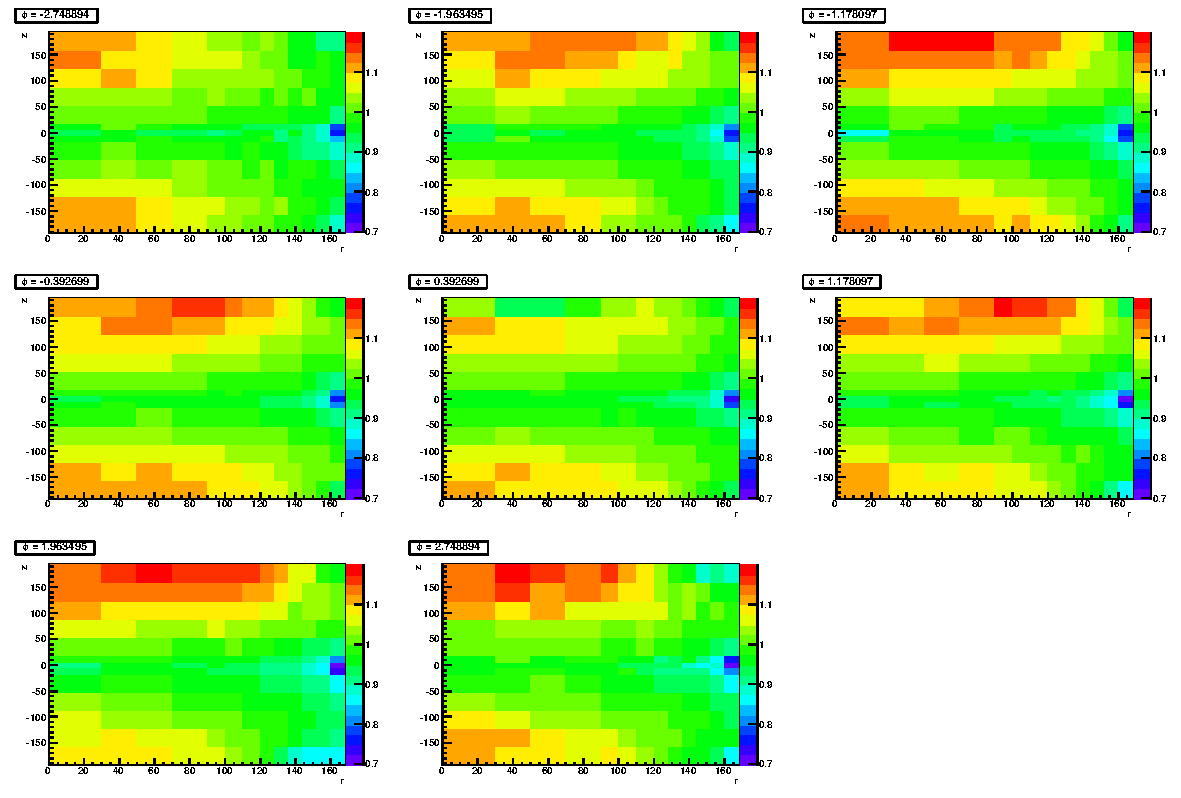
\includegraphics[width=\textwidth]{./plots/lightmap_binned_phi_slices.pdf}
\caption[Lightmap \(\phi\) slices]{The lightmap, showing the bins in \(r\) (horizontal axis) and \(z\) (vertical axis) for each of the 8 \(\phi\) bins.}
\label{fig:lightmap_binned_phi_slices}
\end{figure}
\begin{figure}[tbhp]
\centering
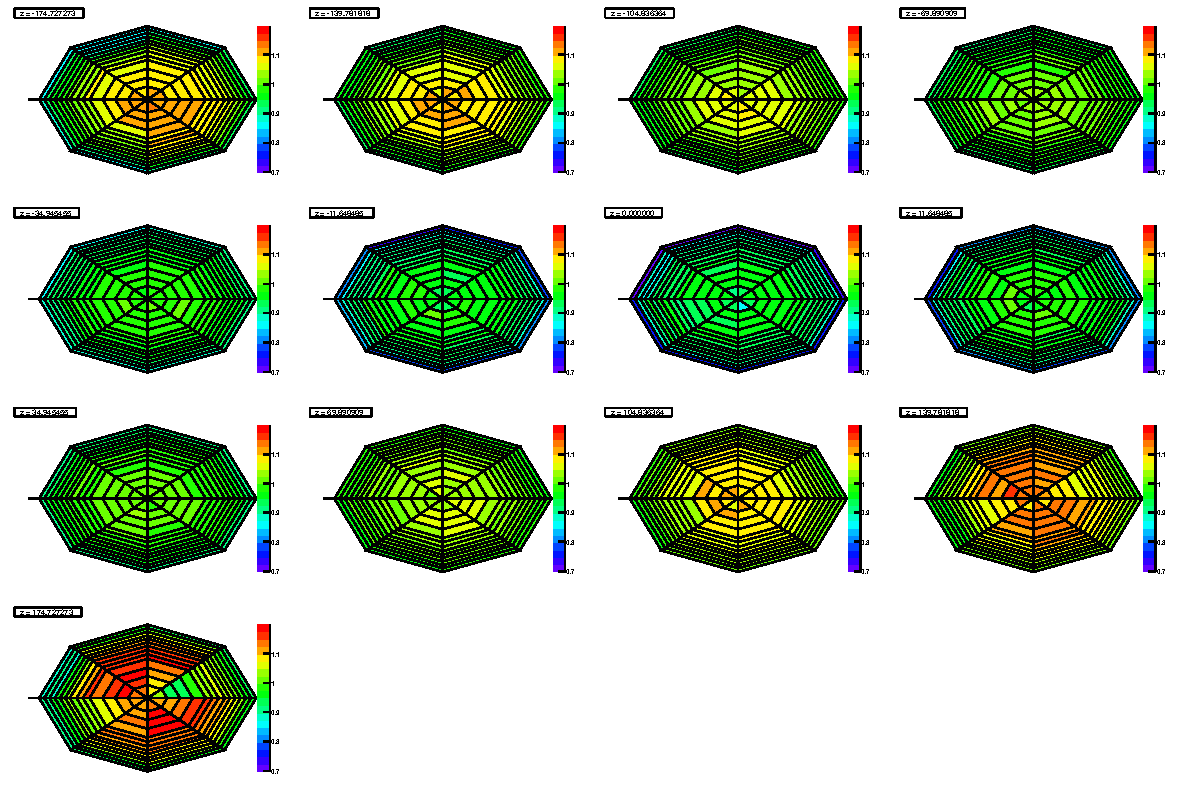
\includegraphics[width=\textwidth]{./plots/lightmap_binned_z_slices.pdf}
\caption[Lightmap \(z\) slices]{The lightmap, showing the bins in \(r\) and \(\phi\) for each of the 13 \(z\) bins.}
\label{fig:lightmap_binned_z_slices}
\end{figure}

The detector volume is divided into 1352 spatial bins. This binning is split into 8 \(\phi\) bins, 13 radial bins, and 13 \(z\) bins. The \(\phi\) binning is evenly-spaced. For the \(z\) binning, the TPC is divided evenly into 11 slices. The central slice is then divided into 3 even slices, since the response is observed to change rapidly near the cathode. The radial binning consists of 1 bin from \SIrange{0}{3}{\mm}, bins every \SI{20}{mm} from \SIrange{30}{90}{\mm}, bins every \SI{10}{\mm} from \SIrange{90}{120}{\mm}, and bins every \SI{8}{mm} from \SIrange{120}{168}{\mm}. This binning is chosen to ensure adequate statistics within all bins, and to optimally map the response in regions with a high light collection gradient.

Full absorption, single site events from all calibrations are placed into the bins according to the event location. Then the mean of each bin is stored in a 3-dimensional histograms. This histogram is referred to as the ``light map'' and is stored in a database. \Cref{fig:lightmap_binned_phi_slices,fig:lightmap_binned_z_slices}\todo{Get new versions of these} shows an example light map. Histograms of the number of events in each bin, and the error on the mean, are also retained to ensure an adequate amount of data was used.

\section{Correction Function}

\end{document}